% =========================================================================
% §6 Results
% Budget: ~2.5 pp
% Drafting order: FIRST (anchors the data narrative).
%
% Layout decisions (locked):
%   - Per-arm aggregates are mean-of-seed-means with across-seed std as the
%     variance estimate (no CIs in body tables).
%   - Localization is reported under View B everywhere; View A is disclosed
%     once in §6.1 and ships under *_view_a columns in the released DB.
%   - Multi-seed (three seeds, pass@1 per seed): all paired tests are
%     Wilcoxon signed-rank (two-sided, normal approximation, no continuity
%     correction) on per-instance pass@1 across seeds. McNemar does not apply
%     because per-instance pass@1 is no longer binary. See analysis/stats.py.
%
% Tables (under tables/):
%   - tab-headline / tab-ablation / tab-per-language
%   - Figures: fig:pareto (§6.1) / fig:firstgold (§6.2) / fig:filecount (§6.3).
%
% Numbers recomputed live by analysis/stats.py + analysis/paper_breakdown.py.
% =========================================================================

\section{Results}
\label{sec:results}

Three arms (SC-ON, SC-OFF, OpenCode) ran Claude Opus 4.7 across three seeds against the
same SWE-PolyBench Verified and SWE-bench-Pro instances. Each subsection states the point
estimate first and follows immediately with the paired-statistics line. Paired tests use
Wilcoxon signed-rank (two-sided, normal approximation) on per-instance pass@1 across the
three seeds; for binary outcomes (resolve, acc@5) per-instance pass@1 lies in
$\{0, 1/3, 2/3, 1\}$, for continuous outcomes (cost, turns, tokens) it is the
per-instance mean. Per-seed values for resolve appear in
Table~\ref{tab:resolve-perseed}; all other metrics are mean of seed means and appear in
Table~\ref{tab:headline}. Acc@5 is reported under View~B throughout; the methodology and
View~A counterpart are disclosed in \S\ref{sec:results-crossharness}.

\subsection{Cross-harness comparison: SC-ON vs.\ OpenCode}
\label{sec:results-crossharness}

\begin{table}[!tbp]
  \centering
  \caption{Resolve \% per seed (seeds 0, 1, 2) for each arm, with the across-seed mean and
    standard deviation. Direction is consistent across seeds for SC-ON over both
    comparators.}
  \label{tab:resolve-perseed}
  % Table: Resolve % by seed for each arm.
% Per-seed resolve for the three seeds (0, 1, 2), with mean and across-seed std.
\begin{tabular}{lccccc}
\toprule
Arm      & Seed 0 & Seed 1 & Seed 2 & Mean & Std \\
\midrule
SC-ON    & 48.8 & 53.6 & 48.8 & \textbf{50.4} & 2.75 \\
SC-OFF   & 43.9 & 41.5 & 40.2 & 41.9          & 1.86 \\
OpenCode & 44.4 & 45.7 & 45.7 & 45.3          & 0.71 \\
\bottomrule
\end{tabular}

\end{table}

\begin{table}[!tbp]
  \centering
  \caption{Headline metrics across the three arms (mean of seed means across three seeds).
    Acc@5 is View~B (agent-targeted); full tables ship in the released results database.
    Turns, tokens, and wall-clock are per-cell means on legit cells.}
  \label{tab:headline}
  % Table 1: Headline metrics across three arms.
% Caption + label live at the \input site in 06_results.tex.
% All numbers are mean of seed means across three seeds (0, 1, 2).
% Acc@5 is View B (DB canonical, loc_metric='agent_targeted_v3').
\begin{tabular}{lccc}
\toprule
Metric & SC-ON & SC-OFF & OpenCode \\
\midrule
Resolve \%                          & \textbf{50.4} & 41.9   & 45.3            \\
Loc acc@5 (View B)                  & \textbf{84.5} & 44.3   & 75.3            \\
Recall@5                            & \textbf{0.611}& 0.330  & 0.601           \\
$\$$/solved                         & \textbf{\$2.30} & \$2.84 & \$2.92        \\
$\$$/cell (mean)                    & \textbf{\$1.15} & \$1.19 & \$1.32        \\
Turns (mean)                        & \textbf{28.3} & 36.2   & 36.0            \\
Tokens, k (mean)                    & \textbf{10.1} & 11.1   & 14.0            \\
Wall-clock, min (mean)              & \textbf{4.5}  & 5.5    & 5.4             \\
\bottomrule
\end{tabular}

\end{table}

Table~\ref{tab:headline} reports the headline metrics for all three arms, and
Figure~\ref{fig:pareto} positions the three arms in the resolve-vs-cost plane: SC-ON
sits upper-left of both comparators, on a cheaper iso-\$/solved curve. Across the three
seeds, SC-ON resolves 50.4\% on average against OpenCode's 45.3\% (paired Wilcoxon on
per-instance pass@1, $n=78$, $\Delta=+6.0$\,pp, $p=0.087$). The direction is consistent
across all three seeds (Table~\ref{tab:resolve-perseed}) but does not separate at the
conventional threshold; the within-harness ablation in \S\ref{sec:results-ablation}
gives the cleanest read.

\begin{figure}[!htbp]
  \centering
  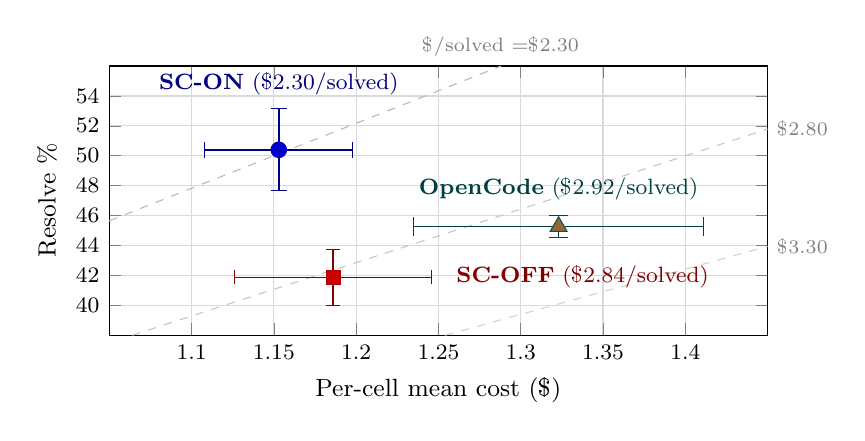
\begin{tikzpicture}
    \begin{axis}[
        width=0.82\linewidth, height=5cm,
        xlabel={Per-cell mean cost (\$)},
        ylabel={Resolve \%},
        xmin=1.05, xmax=1.45,
        ymin=38, ymax=56,
        xtick={1.1, 1.15, 1.2, 1.25, 1.3, 1.35, 1.4},
        ytick={40, 42, 44, 46, 48, 50, 52, 54},
        grid=both, grid style={gray!20},
        major grid style={gray!30},
        tick label style={font=\footnotesize},
        label style={font=\small},
        clip=false,
      ]
      %% Iso-$/solved reference diagonals: resolve = 100 * cost / D
      %% Subtle; the labels carry the cost story, not the lines.
      \addplot[dashed, gray!55, domain=1.05:1.288, samples=2, forget plot] {100*x/2.30};
      \addplot[dashed, gray!45, domain=1.064:1.45, samples=2, forget plot] {100*x/2.80};
      \addplot[dashed, gray!35, domain=1.254:1.45, samples=2, forget plot] {100*x/3.30};
      %% Iso labels: placed where each line exits the visible chart.
      \node[gray, font=\scriptsize, anchor=south] at (axis cs:1.288, 56)  {\$/solved $=$\$2.30};
      \node[gray, font=\scriptsize, anchor=west]  at (axis cs:1.45,  51.8) {\$2.80};
      \node[gray, font=\scriptsize, anchor=west]  at (axis cs:1.45,  43.9) {\$3.30};

      %% Data points: error bars are across-seed standard deviations.
      \addplot+[only marks, mark=*, mark size=2.8pt, color=blue!70!black,
        error bars/.cd, x dir=both, x explicit, y dir=both, y explicit,
        error bar style={blue!50!black, line width=0.6pt}]
        coordinates {(1.153, 50.40) +- (0.045, 2.75)};
      \node[anchor=south, font=\footnotesize, blue!50!black]
        at (axis cs:1.153, 53.4) {\textbf{SC-ON} (\$2.30/solved)};

      \addplot+[only marks, mark=square*, mark size=2.5pt, color=red!70!black,
        error bars/.cd, x dir=both, x explicit, y dir=both, y explicit,
        error bar style={red!50!black, line width=0.6pt}]
        coordinates {(1.186, 41.87) +- (0.060, 1.86)};
      \node[anchor=west, font=\footnotesize, red!50!black]
        at (axis cs:1.255, 41.87) {\textbf{SC-OFF} (\$2.84/solved)};

      \addplot+[only marks, mark=triangle*, mark size=3.5pt, color=teal!70!black,
        error bars/.cd, x dir=both, x explicit, y dir=both, y explicit,
        error bar style={teal!50!black, line width=0.6pt}]
        coordinates {(1.323, 45.27) +- (0.088, 0.71)};
      \node[anchor=south, font=\footnotesize, teal!50!black]
        at (axis cs:1.323, 46.4) {\textbf{OpenCode} (\$2.92/solved)};

    \end{axis}
  \end{tikzpicture}
  \caption{Cost--resolve plane (mean of seed means; error bars are across-seed standard
  deviation). The three dashed lines are iso-\$/solved reference curves (lines of
  constant cost per solve); steeper means cheaper. SC-ON sits on the \$2.30 curve,
  strictly cheaper than SC-OFF (\$2.84, within-harness) and OpenCode (\$2.92,
  cross-harness). The headline cost claim of the paper is the relative position of the
  SC-ON point, not the per-cell mean alone.}
  \label{fig:pareto}
\end{figure}

\textbf{Cost.} SC-ON's \$/solved sits at \$2.30 mean across seeds against OpenCode's
\$2.92 (about 21\% lower). Per-cell mean cost is statistically null (paired Wilcoxon
$p=0.35$); the \$/solved gap is driven by SC-ON's higher resolve rate at comparable
per-cell spend. The substantive claim is that the structural codebase index is not more
expensive to run than agentic grep; on these benchmarks it is favorable.

\textbf{Effort.} SC-ON converges with fewer turns and fewer tokens. Mean turns per cell
are 28.3 for SC-ON against 36.0 for OpenCode (paired Wilcoxon $p<0.0001$); mean tokens
are 10.1k against 14.0k (also $p<0.0001$); mean wall-clock follows at 4.5 against 5.4
minutes. The within-harness ablation in \S\ref{sec:results-ablation} gives the cleanest
mechanism: the index shortens the agent's path to the relevant files, and the saved tool
calls compound into saved tokens and time.

\textbf{Localization.} Acc@5 throughout this paper is View~B (agent-targeted;
\S\ref{sec:design-localization}; the extraction rule is implemented in the released
\texttt{scoring/localization.py}). Under View~B SC-ON acc@5 averages 84.5 across seeds
against OpenCode's 75.3 (paired Wilcoxon $\Delta=+8.1$\,pp, $p=0.080$); under the legacy
View~A the cross-harness comparison shifts (View~A counts engine result-list paths as
files the agent reached, an asymmetry that inflates surfaced sets only for SC-ON). Full
View~A and View~B tables ship in the released results database.

\FloatBarrier
\subsection{Causal ablation: index on vs.\ off}
\label{sec:results-ablation}

\begin{table}[!tbp]
  \centering
  \caption{Causal ablation (SC-ON vs.\ SC-OFF), paired analysis across three seeds. Paired
    tests are Wilcoxon signed-rank (two-sided, normal approximation) on per-instance pass@1
    averaged across seeds. \$/solved is a per-arm aggregate; no paired test applies.
    Acc@5 is View~B.}
  \label{tab:ablation}
  % Table 2: Causal ablation (SC-ON vs SC-OFF), paired analysis across three seeds.
% Pairwise paired-n for ON vs OFF is 80.
% Paired tests use Wilcoxon signed-rank (two-sided, normal approximation) on
% per-instance pass@1 averaged across seeds. $/solved is a per-arm aggregate;
% no paired test applies. Acc@5 is View B (DB canonical).
\begin{tabular}{lcccc}
\toprule
Metric                              & SC-ON          & SC-OFF & $\Delta$                       & Paired $p$ \\
\midrule
Resolve \%                          & 50.4           & 41.9   & $\mathbf{+7.9}$\,\textbf{pp}   & $\mathbf{0.003}$    \\
Loc acc@5 (View B)                  & \textbf{84.5}  & 44.3   & $\mathbf{+39.6}$\,\textbf{pp}  & $\mathbf{<0.0001}$  \\
Recall@5                            & \textbf{0.611} & 0.330  & $\mathbf{+0.281}$              & $\mathbf{<0.0001}$  \\
Turns (mean)                        & 28.3           & 36.2   & $-8.3$                         & $\mathbf{<0.0001}$  \\
Tokens, k (mean)                    & 10.1           & 11.1   & $-1.6$                         & $0.027$             \\
$\$$/cell (mean)                    & \$1.15         & \$1.19 & $-\$0.118$                     & $0.73$ (null)       \\
$\$$/solved                         & \$2.30         & \$2.84 & $-\$0.54$                      & n/a                 \\
\bottomrule
\end{tabular}

\end{table}

Table~\ref{tab:ablation} reports the within-harness ablation. The index is the only thing
that changes between the two arms; model, the rest of the tool set, sandbox, prompts,
seeds, and caps are held fixed.

\textbf{Localization moves substantially.} Under View~B, SC-ON acc@5 averages
\textbf{84.5\%} across seeds against SC-OFF's \textbf{44.3\%} (paired Wilcoxon on
per-instance pass@1, $n=80$, $\Delta=+39.6$\,pp, $p<0.0001$). We use View~B throughout
for the reasons in \S\ref{sec:results-crossharness}. Figure~\ref{fig:firstgold} shows the
discrete CDF behind that point estimate under View~B: the cumulative fraction of legit
cells whose first gold file appears at rank~$\le k$ for $k\in\{1,3,5,10\}$ (the discrete
acc@$k$ values released in the public DB), across all three arms. SC-ON places a gold
file at rank~1 in 77.4\% of cells against SC-OFF's 33.3\%; the gap narrows but does not
close at $k=10$.

\begin{figure}[!tbp]
  \centering
  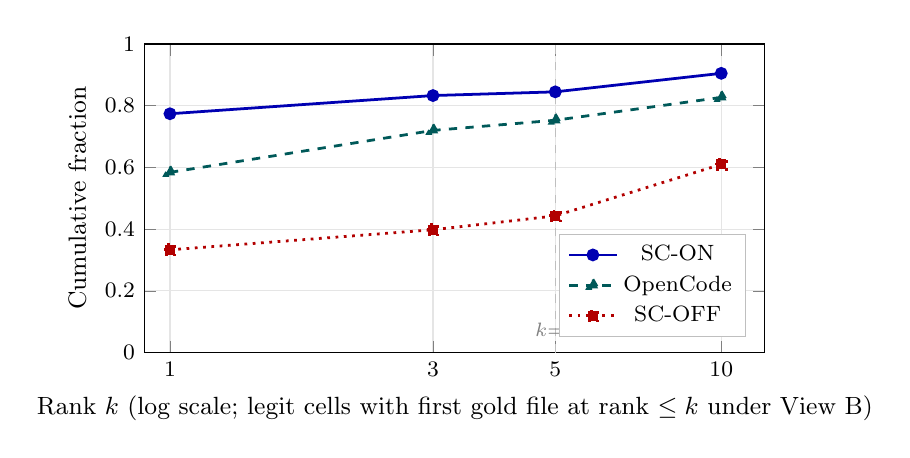
\begin{tikzpicture}
    \begin{semilogxaxis}[
        width=0.78\linewidth, height=5.5cm,
        xlabel={Rank $k$ (log scale; legit cells with first gold file at rank $\le k$ under View~B)},
        ylabel={Cumulative fraction},
        xmin=0.9, xmax=12,
        ymin=0, ymax=1.0,
        xtick={1, 3, 5, 10},
        xticklabels={1, 3, 5, 10},
        ytick={0, 0.2, 0.4, 0.6, 0.8, 1.0},
        grid=major, grid style={gray!20},
        legend style={at={(0.97, 0.05)}, anchor=south east, font=\footnotesize, draw=gray!50},
        tick label style={font=\footnotesize},
        label style={font=\small},
      ]
      %% SC-ON (View B; derived from acc@k columns)
      \addplot[blue!70!black, line width=1pt, mark=*, mark size=1.8pt] coordinates {
        (1, 0.774) (3, 0.833) (5, 0.845) (10, 0.905)
      };
      \addlegendentry{SC-ON}
      %% OpenCode (View B == View A by construction; no engine calls)
      \addplot[teal!70!black, line width=1pt, dashed, mark=triangle*, mark size=2.2pt] coordinates {
        (1, 0.584) (3, 0.720) (5, 0.753) (10, 0.827)
      };
      \addlegendentry{OpenCode}
      %% SC-OFF (View B == View A by construction; no engine calls)
      \addplot[red!70!black, line width=1pt, dotted, mark=square*, mark size=1.8pt] coordinates {
        (1, 0.333) (3, 0.398) (5, 0.443) (10, 0.610)
      };
      \addlegendentry{SC-OFF}
      %% Reference line at k=5 (acc@5)
      \draw[gray!50, dashed] (axis cs:5,0) -- (axis cs:5,1.0);
      \node[gray, font=\scriptsize, anchor=south] at (axis cs:5, 0.02) {$k{=}5$};
    \end{semilogxaxis}
  \end{tikzpicture}
  \caption{First-gold rank CDF under View~B, per arm. Each marker shows the cumulative
  fraction of legit cells (mean of seed means across three seeds) whose first gold file
  appears at rank~$\le k$ in the agent-targeted surfaced set, for the discrete $k$
  values released in the public DB ($k\in\{1,3,5,10\}$). SC-ON dominates at low ranks
  (the regime that matters for the agent's read budget): 77.4\% of cells place a gold
  file at the top, versus 58.4\% (OpenCode) and 33.3\% (SC-OFF). At $k{=}5$ the values
  equal the body acc@5 (84.5 / 75.3 / 44.3) by construction. For OpenCode and SC-OFF,
  View~A and View~B coincide because neither arm makes context-engine calls.}
  \label{fig:firstgold}
\end{figure}

\textbf{Resolve moves with statistical separation.} SC-ON solves 50.4\% of legit cells
on average across seeds against SC-OFF's 41.9\% (paired Wilcoxon $\Delta=+7.9$\,pp,
$n=80$, $p=0.003$). The direction is consistent across seeds. \S\ref{sec:discussion}
reads the three signals together: large localization gain, statistically separated
resolve gain, no per-cell cost regression.

\textbf{Cost and effort.} The index changes how the agent uses tokens, not how much it
costs per cell. Mean turns drop sharply with the index on (28.3 vs.\ 36.2, paired
Wilcoxon $p<0.0001$); mean tokens drop too (10.1k vs.\ 11.1k, $p=0.027$). Per-cell mean
cost is statistically null (paired Wilcoxon $\Delta=-\$0.118$, $p=0.73$); the index buys
fewer turns without a per-cell cost penalty, and \$/solved comes out lower for SC-ON
(\$2.30 vs.\ \$2.84) because of the higher resolve rate at near-equal per-cell spend.

\FloatBarrier
\subsection{Where the index helps: exploratory heterogeneity}
\label{sec:results-heterogeneity}

\begin{table}[!tbp]
  \centering
  \caption{Resolve and View~B acc@5 by language (Go, Java, Python), mean of seed means
    across three seeds. Exploratory; we make no significance claims.}
  \label{tab:per-language}
  \scriptsize
  \setlength{\tabcolsep}{2pt}
  % Table 4: Per-language exploratory stratification (mean of seed means across three seeds).
% acc@5 is View B (DB canonical). Per-language n is per-arm legit
% (ON/OFF/OpenCode), not the manifest count: SC-OFF and OpenCode each lose some
% instances to outcome-blind exclusions (provider_truncation, leak_detected, etc.).
\begin{tabular}{lcccccc}
\toprule
          & \multicolumn{3}{c}{Resolve \%} & \multicolumn{3}{c}{Loc acc@5 (View B)} \\
\cmidrule(lr){2-4} \cmidrule(lr){5-7}
Language ($n_{\text{ON/OFF/OC}}$)  & SC-ON & SC-OFF & OpenCode & SC-ON & SC-OFF & OpenCode \\
\midrule
Go (29/29/31)     & \textbf{47.1} & 29.9 & 35.5 & \textbf{95.4} & 44.8 & 86.0 \\
Java (20/20/19)   & \textbf{60.0} & 53.3 & 57.9 & \textbf{71.7} & 46.7 & 66.7 \\
Python (35/33/31) & \textbf{47.6} & 45.5 & 47.3 & \textbf{82.9} & 42.4 & 69.9 \\
\bottomrule
\end{tabular}

\end{table}

\begin{figure}[!tbp]
  \centering
  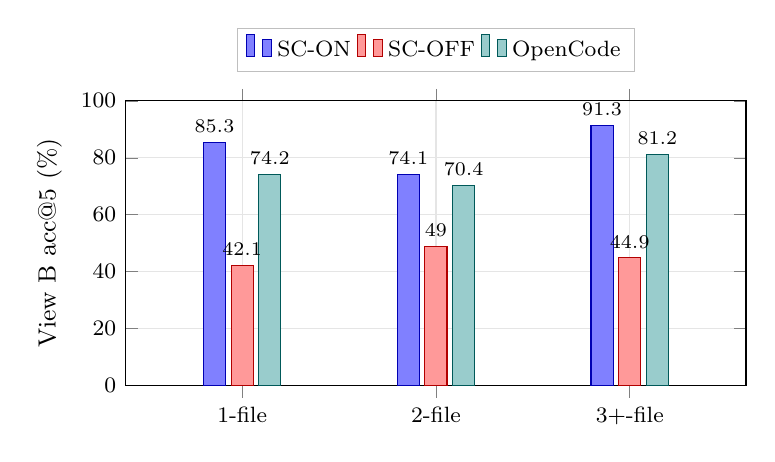
\begin{tikzpicture}
    \begin{axis}[
        width=0.78\linewidth, height=5.2cm,
        ybar, bar width=8pt, enlarge x limits=0.30,
        ylabel={View~B acc@5 (\%)},
        symbolic x coords={1-file, 2-file, 3+-file},
        xtick=data,
        ymin=0, ymax=100,
        ytick={0, 20, 40, 60, 80, 100},
        nodes near coords,
        nodes near coords style={font=\scriptsize, /pgf/number format/precision=1, /pgf/number format/fixed, /pgf/number format/fixed zerofill=false},
        legend style={at={(0.5, 1.10)}, anchor=south, legend columns=3, font=\footnotesize, draw=gray!50},
        tick label style={font=\footnotesize},
        label style={font=\small},
        grid=major, grid style={gray!20},
      ]
      \addplot[fill=blue!50!white, draw=blue!70!black] coordinates {(1-file, 85.3) (2-file, 74.1) (3+-file, 91.3)};
      \addlegendentry{SC-ON}
      \addplot[fill=red!40!white, draw=red!70!black] coordinates {(1-file, 42.1) (2-file, 49.0) (3+-file, 44.9)};
      \addlegendentry{SC-OFF}
      \addplot[fill=teal!40!white, draw=teal!70!black] coordinates {(1-file, 74.2) (2-file, 70.4) (3+-file, 81.2)};
      \addlegendentry{OpenCode}
    \end{axis}
  \end{tikzpicture}
  \caption{View~B acc@5 by gold-file count, mean of seed means across three seeds
  ($n{=}46$, $18$, $27$ distinct instances per bucket respectively). The within-harness
  gap (SC-ON minus SC-OFF) is largest in the 3+\,file bucket
  ($46.4$\,pp) where the call-graph intuition predicts that structural ranking pays
  off more than agentic grep. Exploratory; no significance claims.}
  \label{fig:filecount}
\end{figure}

The slices in this subsection are \emph{exploratory}. Per-language bucket $n$ ranges from
18 to 46. We make no significance claims.

\textbf{By language.} Across seeds, localization gains are largest in Go (View~B acc@5
95.4\% ON vs.\ 44.8\% OFF) and Python (82.9\% vs.\ 42.4\%); Java is more modest (71.7\%
vs.\ 46.7\%). Resolve directionally favors SC-ON in every language: Go 47.1\% vs.\
29.9\%, Java 60.0\% vs.\ 53.3\%, Python 47.6\% vs.\ 45.5\%. On Python, the localization
advantage is substantial (82.9\% vs.\ 42.4\%), narrower than the localization gap
suggests but no longer a directional negative on resolve.

\textbf{By gold-file count.} Figure~\ref{fig:filecount} shows acc@5 across the three
arms split by gold-file count. The index's largest gains sit in the 3+\,file bucket
(91.3\% ON vs.\ 44.9\% OFF), consistent with the call-graph intuition: when the change
spans files, a structural ranking pays off more than agentic grep over the working copy.
Per-bucket resolve is directionally positive for SC-ON in every file-count bucket
(1-file 52.7\% vs.\ 41.3\%, 2-file 55.6\% vs.\ 51.0\%, 3+-file 42.0\% vs.\ 36.2\%).

\FloatBarrier
\subsection{Sensitivity}
\label{sec:results-sensitivity}

Full localization tables under both views ship in the released results database.

\textbf{Localization extractor.} Both views are emitted by the released
\texttt{scoring/localization.py} from the same trace set. The DB's canonical \texttt{acc@k}
columns are View~B; View~A is recomputable locally from traces.
The released \texttt{scoring/localization.py} states the extraction rule precisely.

\textbf{Audit residuals.} The 5 outcome-blind \texttt{git\_history\_leak} cells flagged
in the post-run audit (\S\ref{sec:integrity}) move every headline metric by $\le 1$\,pp
when excluded, and no ranking flips. The network-fetch audit was clean.

\textbf{What we do not claim.} The ON vs.\ OpenCode comparison on resolve and View~B
acc@5 is marginal at multi-seed (paired Wilcoxon $p=0.087$ and $p=0.080$ respectively);
the within-harness ablation is the cleaner read. Across-seed standard deviations are
0.7--3.3\,pp on resolve and acc@5 (consistent with recently-reported coding-agent
benchmark noise floors); the reported ablation effects exceed this noise by 3 to
10$\times$.
\FloatBarrier
